% % % % % % % % % % % % % % % % % % % % % % % % % % % % % % % % % % % % % % % %
% LaTeX4EI Template for Cheat Sheets                                Version 1.1
%
% Authors: Markus Hofbauer
% Contact: info@latex4ei.de
% Encode: UTF-8
% % % % % % % % % % % % % % % % % % % % % % % % % % % % % % % % % % % % % % % %

% ======================================================================
% Document Settings
% ======================================================================

% possible options: color/nocolor, english/german, threecolumn
% defaults: color, english
\documentclass[english]{latex4ei/latex4ei_sheet}

% set document information
\title{HW/SW Codesign \\ Cheat Sheet}
\author{LaTeX4EI}                    % optional, delete if unchanged
\myemail{fabian.olbert@gmail.com}           % optional, delete if unchanged
% \mywebsite{www.latex4ei.de}          % optional, delete if unchanged
\usepackage{float}
\usepackage{amssymb}

% ======================================================================
% Begin
% ======================================================================
\begin{document}
% Title
% ----------------------------------------------------------------------
\maketitle   % requires ./img/Logo.pdf

% Section
% ----------------------------------------------------------------------
\section{Introduction}

\paragraph{Requirements for HW/SW Systems}
\begin{enumerate}
	\item Reliability
	\item Availability
	\item Serviceability
	\item Safety
	\item Efficiency
	\item Real-time capability
	\item Flexibility
\end{enumerate}

\paragraph{Reliability}

\begin{enumerate}
	\item R(t): Probability that a system works correct until time t presuming it worked correct at a reference time $t_0 = 0$
	\item For constant failure rate $\lambda$: $R(t)= e^{-\lambda t} $
	\item \textbf{Metric}: $MTTF = 1 / \lambda$
	\item \textbf{Reliability of Series Systems}: all n components are functional
	\begin{enumerate}
	\item $R_{sys}(t) = R_1(t) \cdot R_2(t)...R_n(t) = \prod_i^n R_i(t)$
	\item Failure probability: $F(t) = 1 - R(t)$
	\item $R_{sys} \leq min(R_i)$
\item 	\end{enumerate}
	\item \textbf{Failure of Parallel Systems}: a single path i is functional
		\begin{enumerate}
			\item $F_{sys}(t) = F_1(t) \cdot F_2(t)...F_n(t) = \prod_i^n F_i(t)$
			\item $R(t) = 1 - F(t)$
		\end{enumerate}

\end{enumerate}

\paragraph{Availability}
\begin{enumerate}
	\item \textbf{A}: Fraction of time the system works correct in between two consecutive failures
	\item $A = \frac{MTTF}{MTBF} = \frac{MTTF}{MTTF + MTTR}$
	\item Metrics: MTBF (Mean Time Between Failures); MTTR (Mean Time to Repair)
\end{enumerate}

\paragraph{Serviceability}
\begin{enumerate}
	\item Measure considering the time it takes to repair a system after a benign
	\item Metric: MTTR 
\end{enumerate}

\paragraph{Abstraction Levels}

\begin{figure}[H]
  \centering
  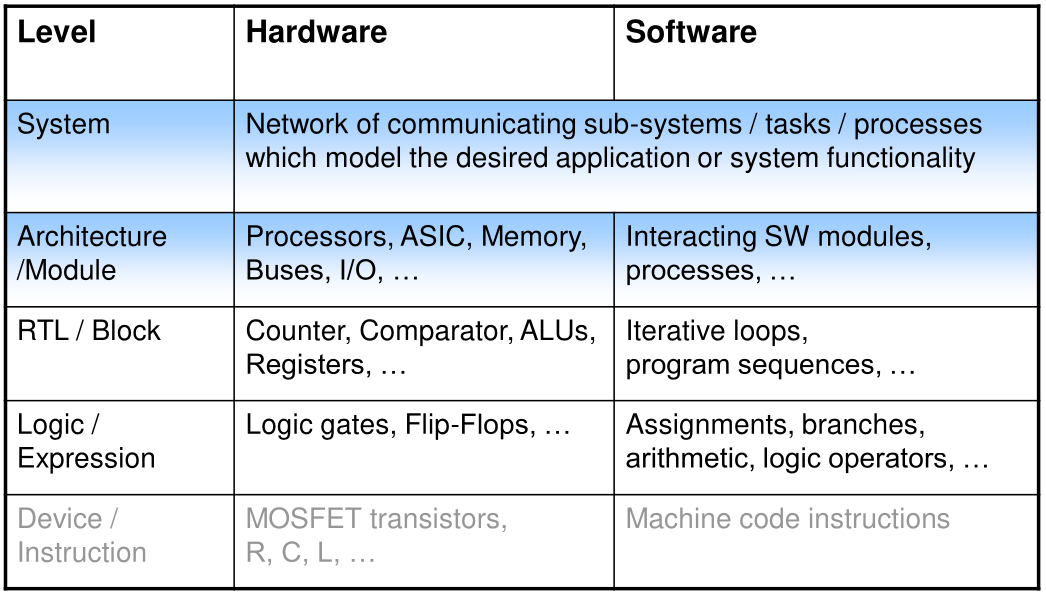
\includegraphics[width=0.8\linewidth]{assets/AbstractionLevels.png}
  % \caption{}
  \label{fig:abstractionlevels}
\end{figure}


\section{Methodology}

\textbf{System Design} is the process to implement a desired function with a given set of physical or software components.

\textbf{Design Flow}: Sequence of individual steps of the design process

\textbf{Top-Down Design}
\begin{enumerate}
		\item \textbf{Specification} of the functional behavior
		\item \textbf{Exploration} of alternative realizations within the design space
		\item \textbf{Refinement} of the most promising realization towards the next lower abstraction level
\end{enumerate}

\paragraph{Specification, Exploration, Refinement}

\begin{center}
  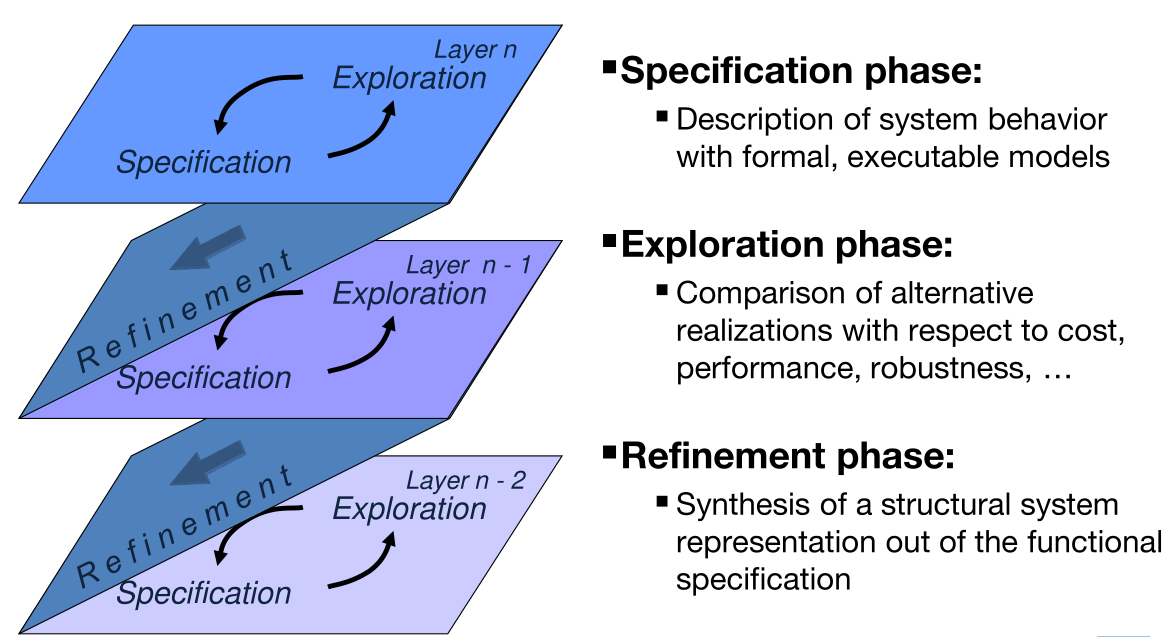
\includegraphics[width=0.8\linewidth]{assets/SpecExRef.png}
\end{center}

\textbf{Abstraction} Design flaws or errors resulting from imprecise modeling or insufficient exploration require abstraction and reiteration of design flow at next higher layer
 
\pragraph{Bottom Up Design}

\begin{center}
  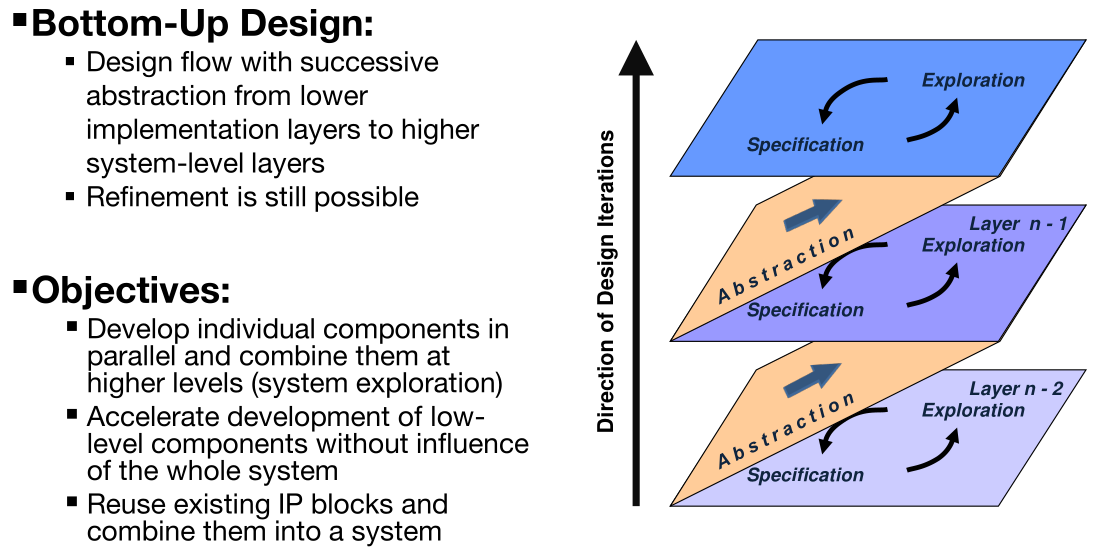
\includegraphics[width=0.8\linewidth]{assets/BottomUpDesign.png}
\end{center}
 
\paragraph{Meet in the Middle Strategy}

\begin{center}
  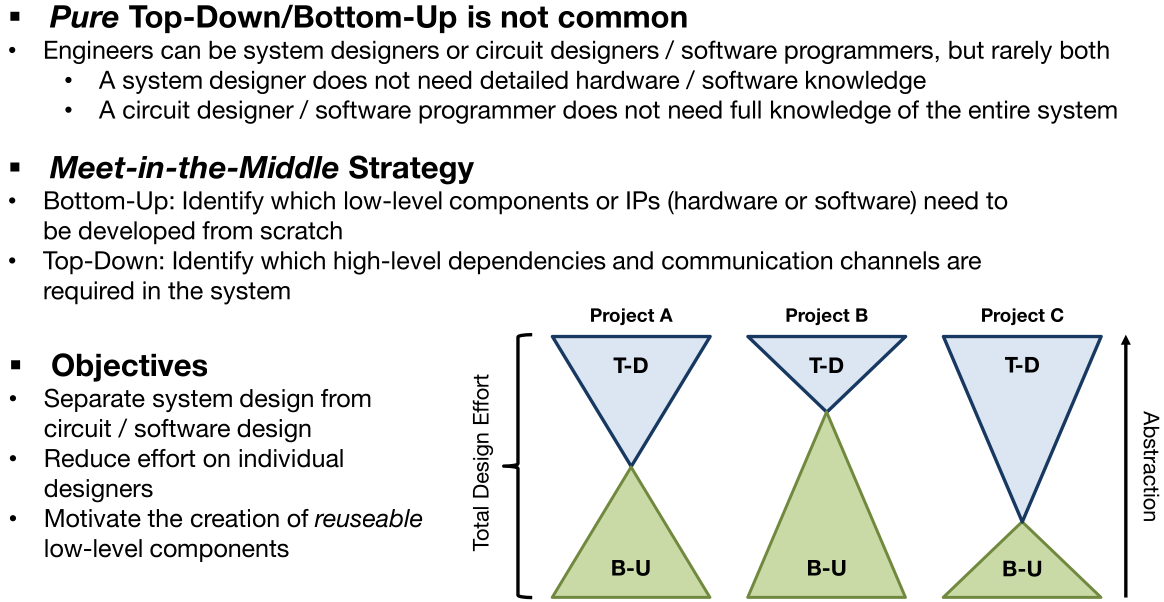
\includegraphics[width=0.8\linewidth]{assets/MeetInTheMiddle.png}
\end{center}

\paragraph{Simulation: Accuracy / Time Effort}

\begin{center}
  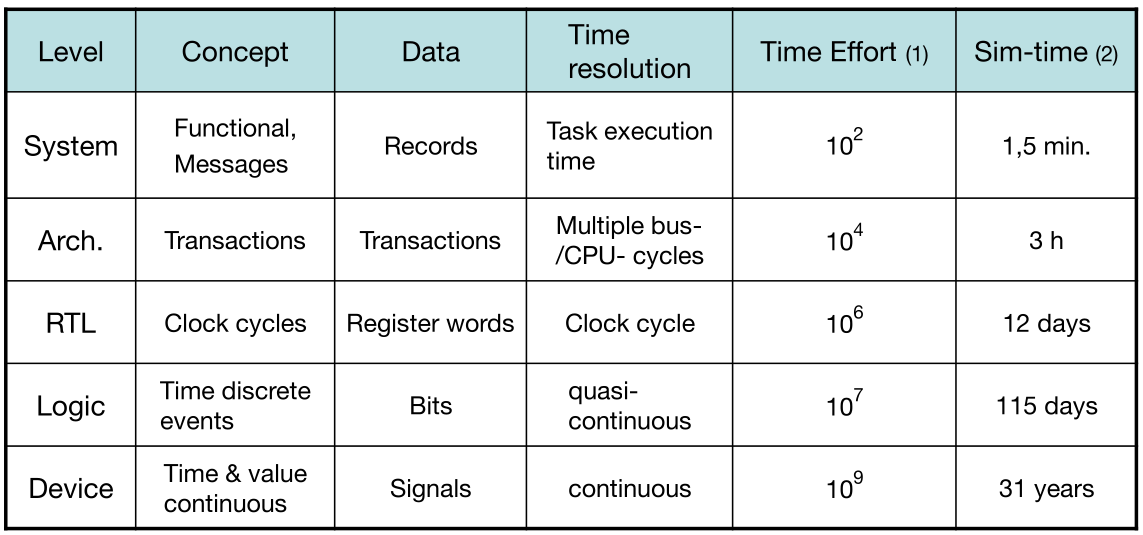
\includegraphics[width=0.8\linewidth]{assets/SimulationAccuracyTime.png}
\end{center}
 
\paragraph{Simualtion Acceleration}
\begin{enumerate}
	\item Divide and Conquer: parallel simulation
	\item Mixed-Level Simulation
\end{enumerate}
 
\paragraph{Design Views}

\begin{center}
  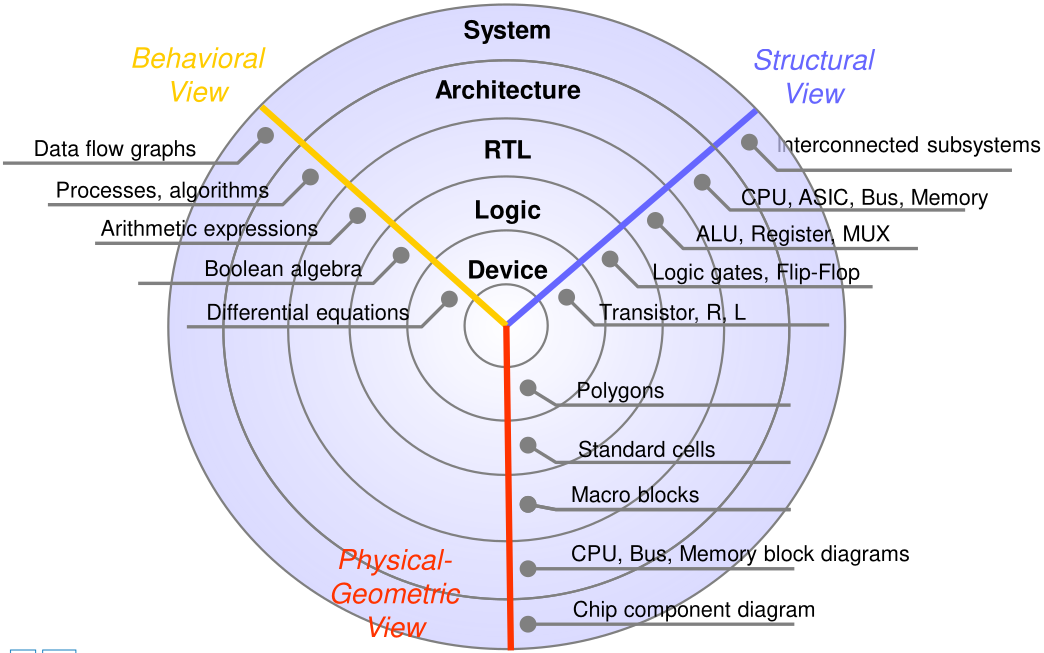
\includegraphics[width=0.8\linewidth]{assets/DesignViews.png}
\end{center}

\paragraph{DesignViewTransition}
\begin{center}
  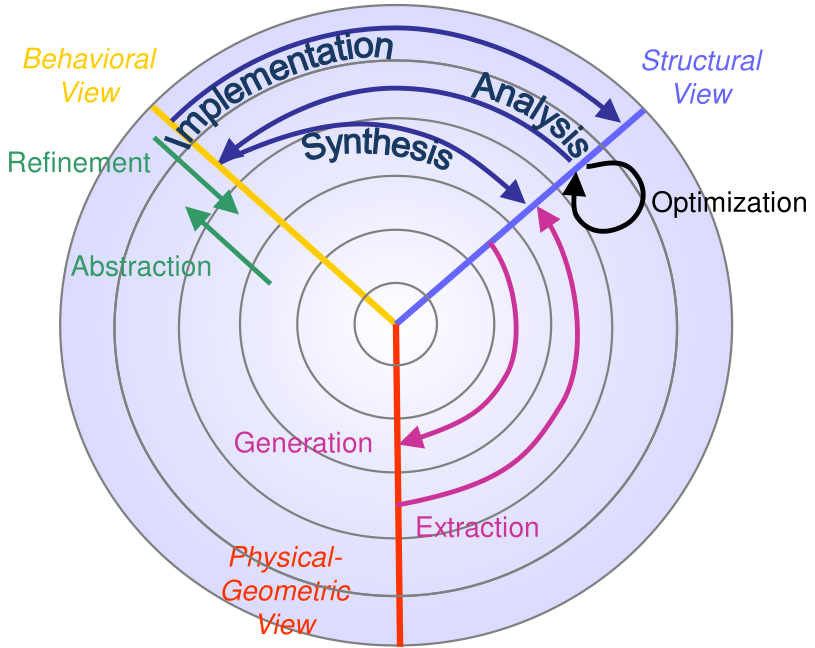
\includegraphics[width=0.7\linewidth]{assets/DesignViewTransitions.png}
\end{center}

\begin{center}
  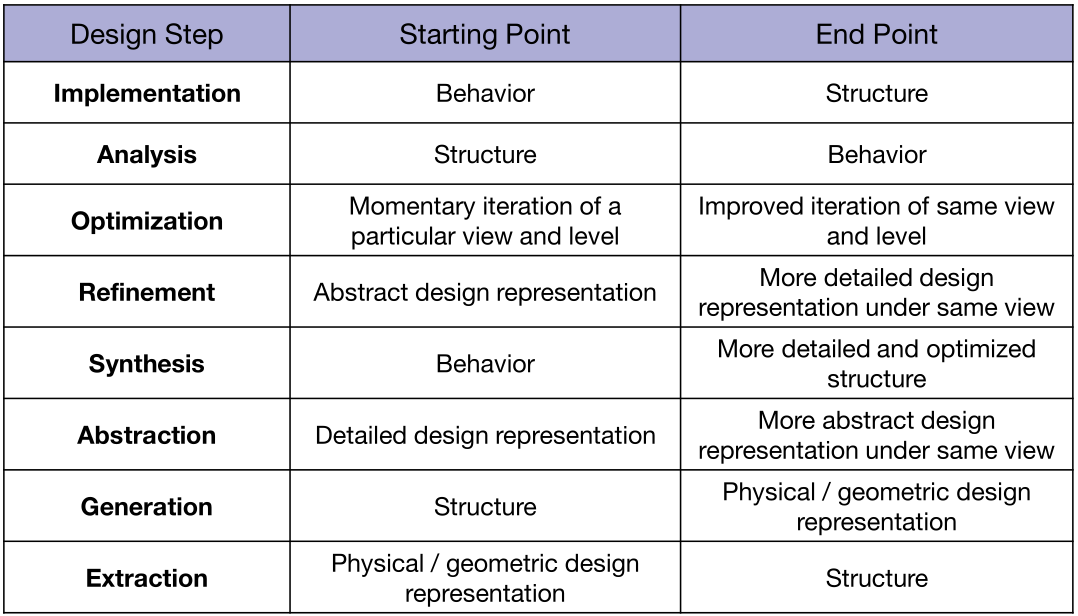
\includegraphics[width=0.8\linewidth]{assets/DesignViewTransitionTable.png}
\end{center}

\begin{center}
  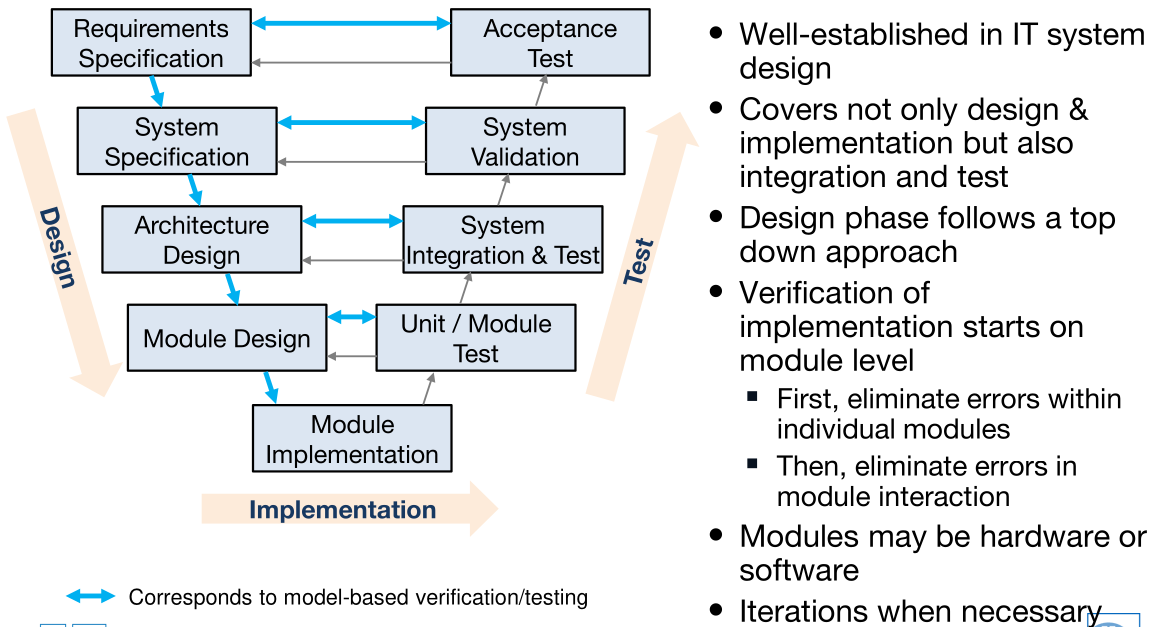
\includegraphics[width=0.8\linewidth]{assets/VModel.png}
\end{center}


\section{Specification \& Modeling}

\begin{center}
  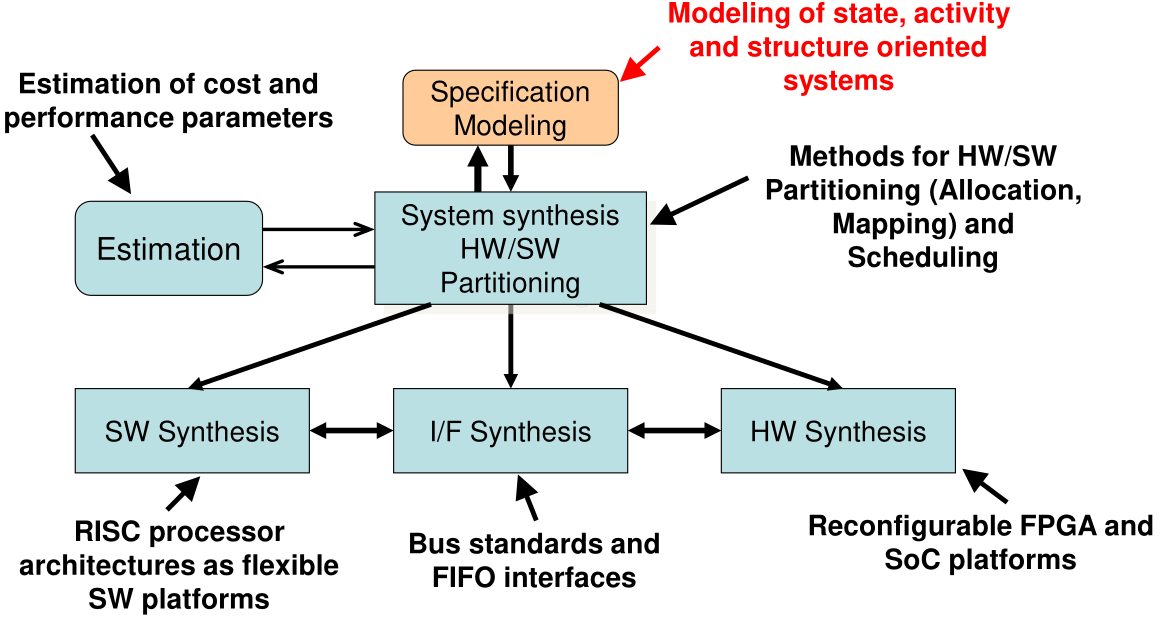
\includegraphics[width=0.8\linewidth]{assets/DesignFlowSystemLevel.png}
\end{center}

\textbf{system specification} defines
\begin{enumerate}
	\item functionality of the system
	\item constrains / properties (latency, power dissipation...)
\end{enumerate}

\section{Synthesis}
\section{Scheduling}
\section{Estimation}



% ======================================================================
% End
% ======================================================================
\end{document}
